\normaltrue \difficilefalse \tdifficilefalse
\correctiontrue 

%\UPSTIidClasse{11} % 11 sup, 12 spé
%\newcommand{\UPSTIidClasse}{12}

\exer{Calcul de moment$\star$ \label{STAT:02:B2:14-gl:516}}
\setcounter{question}{0}\marginnote{\xpComp{STAT}{02}}%\UPSTIcompetence[2]{B2-14}
\index{Compétence STAT-02}
%\index{La Seine Musicale}
\ifcorrection
\else
\marginnote{\textbf{Pas de corrigé pour cet exercice.}}
\fi

\ifprof
\else


\begin{marginfigure}
\centering
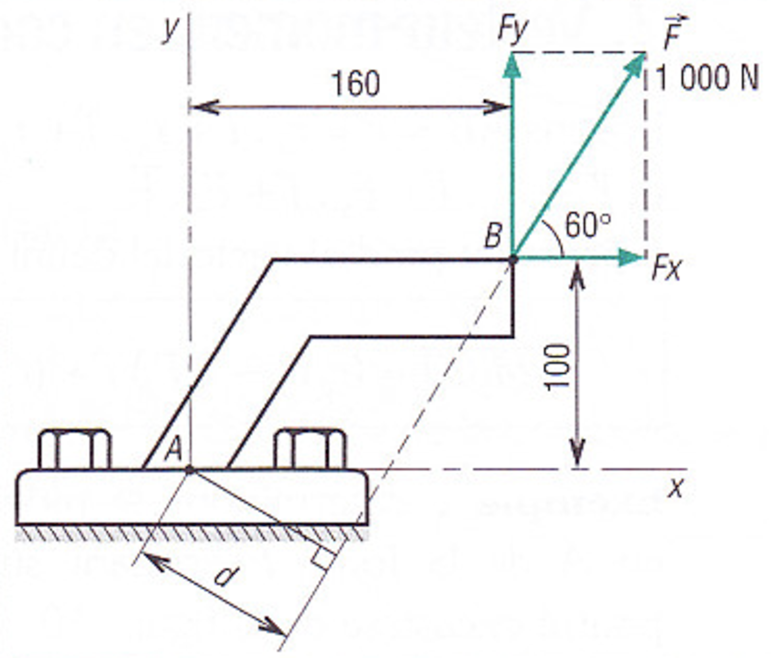
\includegraphics[width=\linewidth]{516_01}
%\caption{Paramétrage de la surface totale et élémentaire en coordonnées sphériques de la demi-voile \label{fig_39_01}}
\end{marginfigure}
\fi


\question{Déterminer $\vect{\mathcal{M}\left(B,F\right)}$.}%\vectm{A}{F}{1}{2}$.}
\ifprof ~\\
On a $\vectm{B}{F}{\text{Bride}} = \vect{0}$
\else
\fi

\question{Déterminer $\vect{\mathcal{M}\left(A,F\right)}$.}%\vectm{A}{F}{1}{2}$.}
\ifprof ~\\
$\vectm{A}{F}{\text{Bride}}=\vectm{B}{F}{\text{Bride}} + \vect{AB}\wedge \vect{F} $ 
$=\left(160 \vx{} + 100 \vy{}\right) \wedge \left(F_x \vx{}+F_y \vy{} \right) $

$= \left(\left(160 \vx{} + 100 \vy{}\right) \wedge  F_x \vx{}+ \left(160 \vx{} + 100 \vy{}\right) \wedge F_y \vy{} \right) $

$= \left( -100 F_x +  160  F_y   \right)\vz{} $
$= \left( -100 \times 1000 \cos 60 +  160   \times 1000 \sin 60 \right)\vz{} $
$= \left( - 50000 +  138 564 \right)\vz{} =  88 564 \vz{} $.
\else
\fi


\ifprof
\else

\marginnote{Corrigé voir \ref{STAT:02:B2:14-gl:516}.}

\fi